This section contains information about the dynamic pricing component.
The component fetches day-ahead prices for the German market and provides these
information to the main system.

\subsection{Day-ahead market service}

We considered multiple different sources for the price information. The following section contains the pros and cons of each source. 
\subsubsection{epexspot.com}
\FloatBarrier
\begin{table}[htbp]
	\centering
	\label{tab:epexspot}
	\begin{tabularx}{\textwidth}{ LLL }
		\toprule
		 Pro & Contra \\\midrule
		\tabitem Website moderate difficult to parse &\tabitem API not free of charge \cite{epexspot} \\
		 \tabitem Lot of useful explanations &\tabitem Not clear if the terms and conditions allow parsing \cite{epexspot}\\
		\bottomrule
	\end{tabularx}
	\caption{Pros and cons of epexspot.com}
\end{table}
\noindent EPEX SPOT provides the day-ahead prices among others for Germany and Luxembourg. The information is directly embedded in the HTML code of the website and does not require JavaScript. As a result of this one could download the website easily, only the parsing part would be harder. Additionally, most changes on the website could lead to adjustments in the parsing code. Moreover, they provide an API but it is expensive to use and the terms and conditions are not clear if it is allowed to parse the site. \Cref{tab:epexspot} provides an overview of the pros and cons.
\FloatBarrier

\subsubsection{nordpoolgroup.com}
\FloatBarrier
\begin{table}[htbp]
	\centering
	\begin{tabularx}{\textwidth}{ LLL }
		\toprule
		Pro & Contra \\\midrule
	     \tabitem Lot of Nordic countries & \tabitem No day-ahead prices for Germany \cite{nord}\\
		 &\tabitem You need to be a customer to use the API \cite{nord}\\
		  &\tabitem Harder to parse the website\\
		 &\tabitem Automatic data extraction not allowed in the terms and conditions \cite{nord2}\\ 
		\bottomrule
	\end{tabularx}
	\caption{Pros and cons of nordpoolgroup.com}
	\label{tab:nordpoolgroup}
\end{table}

\noindent Nord Pool AS provides day-ahead prices for a lot of Nordic and other countries \cite{nord0}. Data is provided for example for the UK, Norway or Sweden. But Germany is not included. Additionally, the website does not directly contain the data and requires JavaScript to fetch them. So parsing is harder and not allowed in the terms and conditions \cite{nord2}. They have an API but it is only available to customers \cite{nord}. \Cref{tab:nordpoolgroup} provides an overview of the pros and cons of Nord Pool AS as a data source.
\FloatBarrier
\subsubsection{smard.de}
\FloatBarrier
\begin{table}[htbp]
	\centering
	\begin{tabularx}{\textwidth}{ LLL }
		\toprule
		Pro & Contra \\\midrule
 \tabitem Data licensed under CC BY 4.0 \cite{Bundesnetzagentur} &\tabitem No API\\
 \tabitem Fast support &\tabitem Support discourages parsing of the website\\
		\bottomrule
	\end{tabularx}
	\caption{Pros and cons of smard.de}
	\label{tab:smard}
\end{table}

\noindent Smard.de is provided by the German Bundesnetzagentur. They provide data for Germany and Luxembourg (combined bidding zone). They provide the data licensed under CC BY 4.0 \cite{Bundesnetzagentur}. Additionally, they have a fast and friendly support. But they do not offer an API and the support said that they do not want automatic data extraction on the website. So we did not check if it is feasible. See \Cref{tab:smard} for a short recap.

\FloatBarrier
\subsubsection{dataminer2.pjm.com}
\FloatBarrier
\begin{table}[htbp]
	\centering
	\begin{tabularx}{\textwidth}{ LLL }
		\toprule
		Pro & Contra \\\midrule
		 \tabitem API available \cite{dataminer} &\tabitem Does not provide data for Germany \cite{dataminer}\\
		&\tabitem API requires an account\cite{dataminer}\\
		\bottomrule
	\end{tabularx}
	\caption{Pros and cons of dataminer2.pjm.com}
	\label{tab:dataminer2}
\end{table}
\noindent The Data Miner 2 from PJM provides an API but it does not provide data for Germany \cite{dataminer}. So we did not investigate this data source any further. As always \Cref{tab:dataminer2} contains the pros and cons.

\FloatBarrier
\subsubsection{transparency.entsoe.eu}\label{subsubsec:entsoe}
\begin{table}[htbp]
	\centering
	\begin{tabularx}{\textwidth}{ LLL }
		\toprule
		Pro & Contra \\\midrule
		 \tabitem Free API \cite{ENTSO} &\tabitem API parameters use non standard formats\\
		 \tabitem Has data for Germany &  \\
		 \tabitem Terms and conditions allow free usage of data \cite{ENTSO2} & \\
		 \tabitem Fast and helpful support \cite{ENTSO2} & \\
		\bottomrule
	\end{tabularx}
	\caption{Pros and cons of transparency.entsoe.eu}
	\label{tab:entsoe}
\end{table}
\noindent ENTSO-E provides the day-ahead prices for a lot of countries. Germany is among them. Additionally, the Transparency Platform provides a free REST API with documentation \cite{ENTSO}. Some of the parameters of the API use non-standard formats, but it is still usable. The data provided by the API can be used freely \cite{ENTSO2}. We also had contact with the support and the replies were fast and friendly. \Cref{tab:entsoe}  summarizes the pros and cons.

\subsection{Conclusion}

We reviewed five data sources and only one provides data for Germany and has a free API. As a result of this, we decided that we use the service from ENTSO-E (\Cref{subsubsec:entsoe}). You have to request a security token from their support, but they replay fast. The data return by this API are the prices for Germany and Luxembourg because this is a combined bidding zone.

\subsection{Price collector component}
\begin{figure}[htpb]
	\centering
	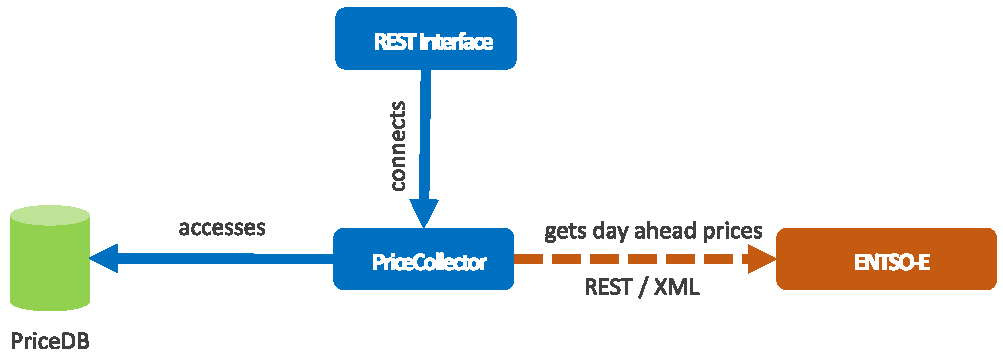
\includegraphics[width=1.00\textwidth]{../figures/priceCollector.pdf}
	\caption{Components: Price Collector}
	\label{fig:price}
\end{figure}
\noindent To fetch the data, we implemented an additional component which communicates with the API from ENTSO-E and manages database to store the data. \Cref{fig:price} contains an overview of the components used in your price collector. The price collector offers a REST Interface which uses JSON for the communication with the rest of our system. It communicates via an XML Format with the ENTSO-E REST Interface. It reads the data items from the API, filters them for the for us relevant data and saves them in an H2 Database. The necessary security token, the bidding zone and the port for the interface can be configured in a configuration file. The price collector has an auto-fetch feature which is also configurable and allows to request the ENTSO-E API in a user-defined pattern. For example, the day-ahead prices are published between 12 pm and 1 pm (one hour after gate closure) \cite{ENTSO3}. So it is possible to update the database each day at 1 pm. But also, more or less frequent patterns are possible. For example, each second hour. The price collector always tries to update its data with each request. If the ENTSO-E API is not available or it does not provide data for a specific period, the price collector uses older but still the most recent data from the database to fill the gaps. For example, if you request data for tomorrow at 4 pm and there is no data available from ENTSO-E the price collector will return the data from today at 4 pm. Such old data will be marked with a boolean flag in the response.    



\noindent We also updated your main architecture to reflect the new requirements. \Cref{fig:updatedA} showed the new architecture with the price collector. The database from the price collector is omitted in this figure. The Controller communicates via HTTP with the REST interface of the price collector. The price collector only offers one endpoint which is \glqq/prices\grqq{}. To make a request the start time and the end time of the required period have to be provided via query parameters. For all time-related information, the time zone UTC is used. 

\begin{figure}[htpb]
	\centering
	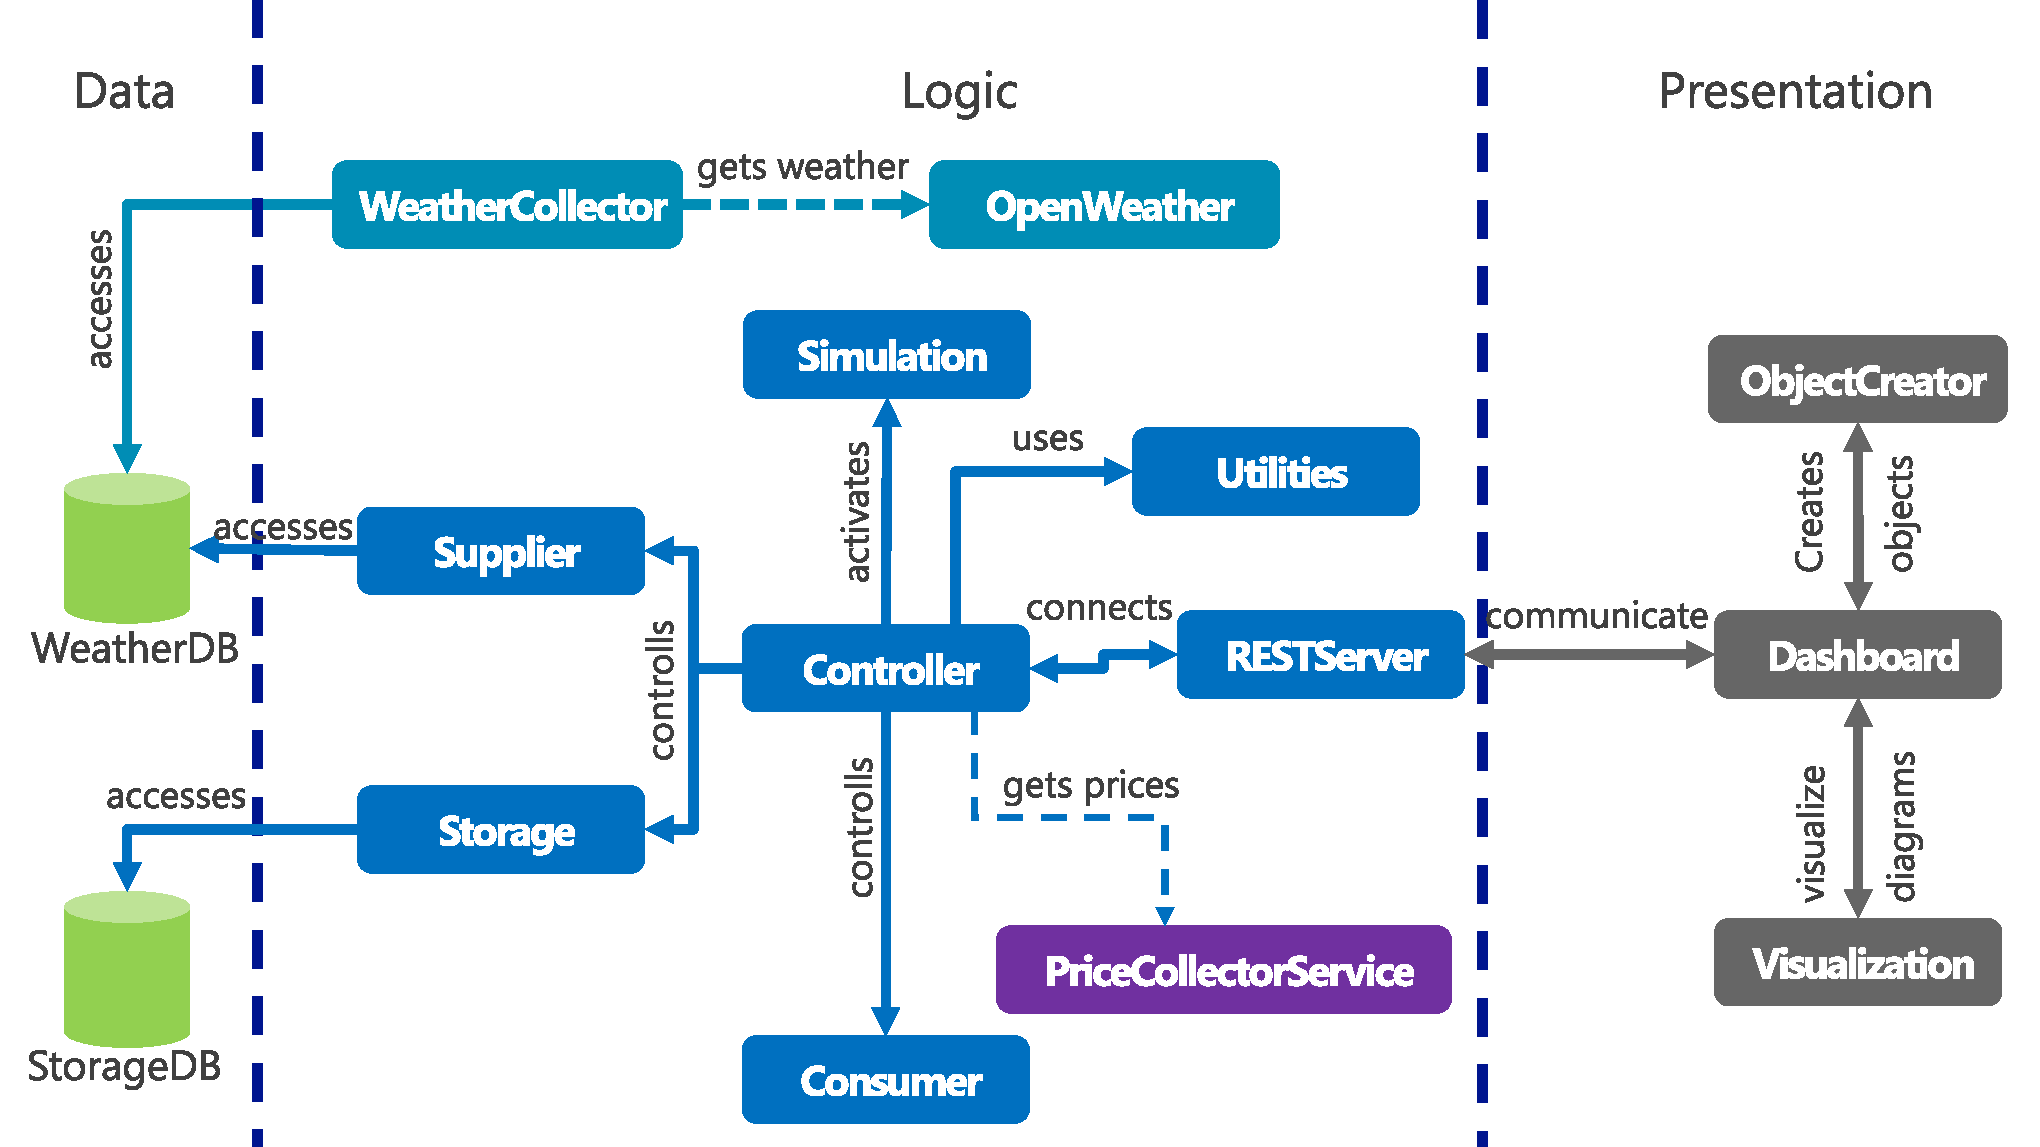
\includegraphics[width=1.00\textwidth]{../figures/Architecture2.pdf}
	\caption{Components: Price Collector}
	\label{fig:updatedA}
\end{figure}

\noindent The following figure contains an example snippet from an answer of our service. To use this answer our main system has to convert the information into the correct units. As always we provide a swagger documentation in the running competent.  

\begin{figure}[htpb]
	\centering
	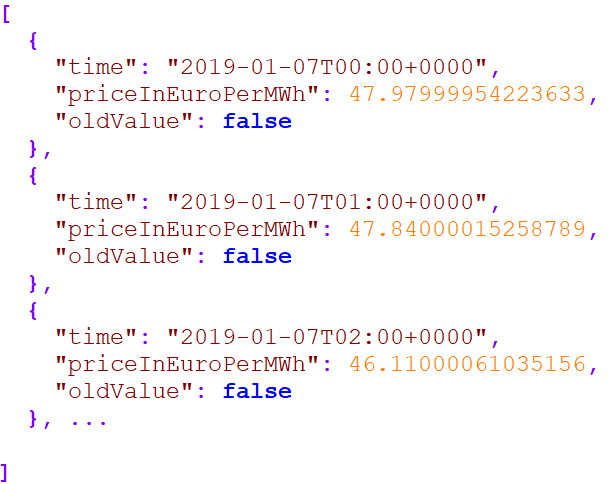
\includegraphics[width=0.5\textwidth]{../figures/response.png}
	\caption{Example response snippet}
	\label{fig:snipped}
\end{figure}
 
\noindent With this component, our system can simulate a microgrid and use real price data. We also added a test script to our repository to test the whole system. 
 \FloatBarrier